\chapter{Phase d'analyse~: des besoins aux fonctionnalités}
	\paragraph{}
	La partie précédente était consacrée à l'explication des notions qui nous
	seront indispensables pour la suite. Nous avons vu
	ce qu'est un EAI et les enjeux de la supervision. Nous avons également vu que
	TrackCIS est une console de supervision et que notre projet vise à l'améliorer.
	L'objectif de cette deuxième partie est de décrire aussi précisément que
	possible la solution à développer. Pour cela, il nous faut comprendre les
	besoins des utilisateurs, les traduire en
	fonctionnalités et modéliser les comportements de la solution à développer.
	
	\section{L'enquête permet une meilleure compréhension des besoins des utilisateurs}
		\paragraph{}
		Un besoin est formulé par le destinataire d'une application, l'utilisateur. Il
		peut l'être explicitement ou implicitement. Pour collecter ces besoins, nous
		allons interroger un certain nombre d'utilisateurs.
		
		\subsection{Élaboration d'un questionnaire d'enquête et conduite des entretiens}
			\paragraph{}% Les objectifs de l'enquêtes
			Les trois objectifs de cette enquête sont~:
			\begin{itemize}
			  \item Etablir une liste de besoins
			  \item Comprendre comment sont supervisés les flux, ce qui implique~:
			  \begin{itemize}
			    \item de savoir comment sont
			  	organisés les DSIO (Direction des services informatiques et de
			  	l’organisation) des établissements hospitaliers pour mieux comprendre qui
			  	s'occupe de la supervision
			  	\item de connaître les pratiques actuelles des personnes en charge de la
			  	supervision
			  	\end{itemize}
			  \item Connaître les utilisateurs de TrackCIS et plus généralement dresser
			  un profil des utilisateurs des consoles de supervision
			\end{itemize}
			
			\paragraph{}% Les principes de l'étude qualitative
			Il s'agit d'une étude qualitative. Contrairement aux études quantitatives qui
			permettent de récolter des données repérsentatives d'une population, dans une
			étude qualitative nous ne cherchons pas à interroger le plus de personnes
			possibles \citep{alami_les_2009}. Les entretiens sont basés sur des questions
			ouvertes et durent en général plus longtemps que dans pour les enquêtes
			quantitatives, une trentaine de minutes dans notre cas.
			L'objetcif est de faire ressortir la diversité des comportements, des
			pratiques.\newline
			Les entretiens sont conduits de manière semi-directive par téléphone ou en
			face à face quand cela est possible.
			Le questionnaire n'est qu'une trame aidant à orienter la discussion. Il a
			vocation à évoluer d’un entretien à l'autre. Des questions peuvent être
			modifiées, supprimées ou ajoutées de façon à obtenir des informations de plus en
			plus pertinentes (l'annexe A présente la dernière version du guide
			d'entretien).
			Chaque entretien donne lieu à un compte-rendu détaillé dont la structure reprend
			la trame du
			questionnaire. L'annexe B présente de manière exhaustive l'ensemble
			des compte-rendu des entretiens.\newline
			Voici le plan de notre
			questionnaire~:
			\begin{itemize}
			  \item[1) Identification de la personne, exploration du contexte~:] Quels
			  sont les responsabilités et les fonctions de la personne et de son
			  service~? Comment celui-ci est-il organisé~?
			  \item[2) Utilisations et utilisateurs de Cloverleaf et problématique de la
			  supervision des flux~:] Qui est en charge de Cloverleaf et comment~?
			  \item[3) Attentes par rapport aux consoles de supervision~:] Qu'est-ce
			  qu'une bonne console de supervision ? En quoi consiste la supervision~?
			  \item[4) Les consoles actuelles~:] Comment les consoles actuelles
			  sont-elles utilisées~? Quelles sont les avantages et les inconvénients des
			  outils existants~? L'affichage de statistiques est-il pertinent~?
			\end{itemize}
			
			\paragraph{}% Choix de la population interrogée
			Un panel de cinq établissements hospitaliers est interrogé. Tous ces
			établissements sont des clients d’Xperis (tableau \ref{panel_enquete}) mais
			n'utilisent pas forcément TrackCIS (car ils ne l'ont pas acheté ou ne
			l'utilisent tout simplement pas).
			\begin{table}[H]
				\centering
				\caption{\label{panel_enquete} Description du panel interrogé}
				\begin{tabular}{| p{3cm} | p{5cm} | p{5cm} |}
					\hline
						\thead{Etablissement}
						&\thead{Utilisateur de TrackCIS ?}
						&\thead{Personne interrogée}
						\\
					\hline
						Tours
						&
						Oui, mais la console est actuellement peu utilisée.
						&
						Personne de l'équipe qui est en charge des différents EAI de
						l'établissement.
						\\
					\hline
						Metz
						&
						Oui, au quotidien.
						&
						Responsable de l'exploitation (chargé de la surveillance des flux).
						\\
					\hline
						Brest
						&
						Non.
						&
						Trois responsables de l'interopérabilité ayant une bonne maîtrise de
						Cloverleaf.
						\\
					\hline
						Rouen
						&
						Oui, mais la console est actuellement peu utilisée.
						&
						Personne de l'équipe qui est en charge des différents EAI de
						l'établissement.
						\\
					\hline
						Toulouse
						&
						Oui.
						&
						Responsable intégration et urbanisation.
						\\
					\hline
				\end{tabular}
			\end{table}
			
			\paragraph{}% Méthodes d'analyse des résultat
			A l'issue des entretiens, après une rapide relecture de tous les comptes
			rendus d'entretien, nous établissons une liste des grands thèmes qui ont été
			abordés durant les discussions \citep{alami_les_2009}.
			On classe ensuite chaque information collectée dans l'un de ces
			thèmes.\newline Les grands thèmes en question sont les suivants~:
			\begin{itemize}
			  \item[1)] L’organisation des services informatiques dans les
			  hôpitaux
			  \item[2)] Les types d’utilisateurs de TrackCIS
			  \item[3)] Les types d’utilisations de TrackCIS
			  \item[4)] Les attentes par rapport aux consoles de supervision
			  et la réponse des outils actuels à ces attentes
			  \item[5)] Les fonctionnalités manquant aux consoles de
			  supervisions actuelles
			  \item[6)] Les statistiques sur les flux
			\end{itemize}
			Dans la suite de cette partie nous entrerons dans le détail des informations
			collectées pour chacun de ces grands thèmes.
			
		\subsection{La supervision fait partie du processus de résolution des
		anomalies}
			\paragraph{}% L'organisation des DSIO
			Les services informatiques ont des structures très variables selon les
			établissements. Cependant, il existe dans tous les cas observés au moins un
			département consacré à l’interopérabilité. Il peut se subdiviser
			en deux pôles~:
			\begin{itemize}
			  \item Un pôle intégration
			  \item Un pôle exploitation
			\end{itemize}
			\textbf{Le pôle intégration} prend en charge la mise en place de nouveaux
			flux et du bon fonctionnement de l’EAI en général. Son niveau de compétence sur
			Cloverleaf est élevé. Ce pôle existe dans des établissements
			relativement autonomes vis-à-vis des éditeurs de logiciels. Le pôle
			intégration se compose généralement de deux ou trois personnes. Les outils
			utilisés sont principalement l’IDE, et des consoles de supervision telles que EAI
			Supervision ou Global Monitor.\newline
			\textbf{Le pôle exploitation} a en charge la supervision des flux. Le niveau
			de maîtrise de Cloverleaf y est plus faible. Les outils utilisés sont en
			général, les différentes consoles de supervision,
			mais rarement l’IDE, trop complexe pour ce type d’utilisateur.\newline
			Les deux pôles peuvent cohabiter au sein d’un même établissement. Certains,
			comme le CHU (Centre hospitalier universitaire) de Metz, n’ont qu’un pôle
			exploitation, la mise en place des flux étant assuré par un autre département (en l’occurrence, le département
			en charge de l’urbanisation du SI). D’autres établissements, beaucoup plus
			dépendants des éditeurs, ne s’occupent pas de la mise en place des flux ni
			du fonctionnement de l’EAI, mais seulement de la supervision. C’est par
			exemple le cas du CH de Châtellerault.\newline
			Il y a différents niveaux de gestion de l’interopérabilité au sein d’un
			hôpital.
			Les niveaux correspondent au degré de responsabilité vis à vis de
			l'interopérabilité. Plus un niveau est élevé, plus les impacts des
			décisions prises à ce niveau seront forts sur le SI. Un pôle exploitation se
			situe au niveau le plus bas tandis qu’un pôle intégration peut se situer au
			niveau deux ou trois. Le niveau le plus haut est en général assuré par un
			département urbanisation, en charge de la définition de la politique de tout le SI.
			
			\paragraph{}% Diversité des pratiques
			L’ensemble des outils liés à Cloverleaf (IDE et consoles)
			peut être utilisé pour la supervision des flux. Les utilisateurs les plus
			aguerris sur Cloverleaf utilisent l’IDE, notamment une fonctionnalité,
			nommée \textit{status} qui donne accès à des données statistiques sur un
			thread ou un process à un instant t. Pour détecter les problèmes,
			l’utilisateur se fie principalement à la date et à l'heure de dernière
			écriture d’un message sur le flux. Si rien n’a été écrit depuis un certain temps, c’est que
			le flux est bloqué et que les messages ne passent plus. Ce type d’utilisateur
			fait généralement partie du pôle intégration et est en charge de la
			résolution des problèmes les plus complexes.
			Pour cela, il a parfois recours à des fonctionnalités avancées comme la
			consultation de la base de données d'erreurs (ou \textit{error database}) ou
			de la base de données contenant les messages (ou \textit{SMAT database})
			pour remonter à l’origine de l’erreur.\newline
			Du côté des consoles de supervision, les principaux usages sont~:
			\begin{itemize}
			  \item Visualiser l’état des flux, c'est-à-dire vérifier que les threads et
			  process fonctionnent correctement,
			  \item Affichage sur écran géant,
			  \item Rechercher un message en particulier, ou un certain type de
			  message. Par exemple, tous les messages concernant un patient donné ou
			  qui sont passés à une date donnée,
			  \item Visualiser les messages qui sont en erreur,
			  \item Supervision en mode lecture seule~: permet de faire remonter les
			  erreurs aux personnes ayant les compétences pour les résoudre,
			  \item Lire le contenu d'un message pour diagnostiquer une erreur,
			  \item L'éditer pour corriger l'erreur quand celle-ci est causée par le
			  message, puis rejouer le message,
			  \item Réaliser des tests lors de la mise en place de flux (usage repéré
			  uniquement au CHU de Toulouse),
			  \item Pour les flux entre les applications de l'éditeur Maincare
			  uniquement, s’assurer que les messages soient bien intégrés dans les
			  applications destinatrices,
			  \item Restreindre l’utilisation de certaines fonctionnalités pour par
			  exemple confier les outils à des personnes d’astreintes ou à des personnes
			  métiers,
			  \item Comparer le contenu d’un message à l'entrée et à la sortie d'un flux.
			  \item Paramétrer l’outil~: création de colonnes, attribution des droits…
			\end{itemize}
			\paragraph{}
			L’utilisation la plus simple des consoles est la visualisation (figure
			\ref{usage_consoles})~: voir les messages qui passent et pouvoir détecter
			rapidement les erreurs. Une fois détectées, l’utilisateur cherche à
			comprendre ce qui les a causées. Pour cela, il peut être suffisant de
			regarder le contenu du message pour en repérer les anomalies, ou bien faire
			des recherches plus complexes.
			Une fois le diagnostic fait, il faut corriger le problème. Ceci peut se
			faire par édition du contenu du message puis par rejoue, dans les cas les
			plus simples.\newline
			Les utilisateurs les plus
			avertis ont en charge l’administration de la console, c’est-à-dire son
			paramétrage (attribution des droits de consultation et d’action aux
			utilisateurs, paramétrage des données affichées\ldots). Ce rôle revient
			généralement au pôle intégration, aux éditeurs ou à Xperis.
			\begin{figure}[H]
				\centering
				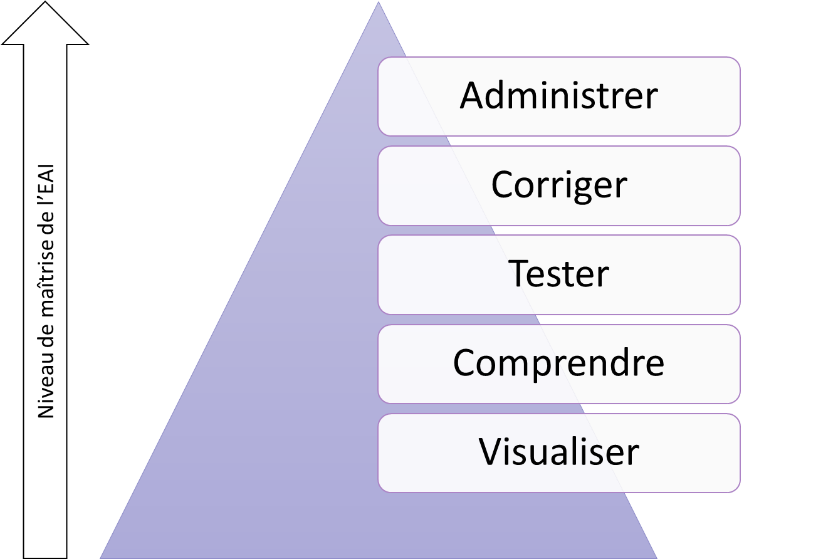
\includegraphics[width=10cm]{../img/usage_1.png}
				\caption{\label{usage_consoles} Les différentes utilisations des consoles
				de supervision}
			\end{figure}
			
			\paragraph{}
			Nous pouvons définir la supervision d'un flux comme~:
			\begin{itemize}
			  \item Pouvoir détecter en un coup d’œil la présence d’anomalies telles que
			 ~:
			  	\begin{itemize}
			  	  \item Des erreurs,
			  	  \item Des ralentissements,
			  	  \item Des blocages
		  	    \end{itemize}
			  \item Pouvoir expliquer, même partiellement ces anomalies,
			  \item Et éventuellement pouvoir agir dessus dans le but de les corriger.
			  Cependant, selon deux des cinq personnes interrogées le but premier d'une
			  console n'est pas la correction mais seulement la détection des anomalies. 
			\end{itemize}
			
		\subsection{Une grande diversité des utilisateurs des consoles de
		supervision}
			\paragraph{}% Les utilisateurs
			Nous pouvons établir une typologie des utilisateurs des consoles de
			supervision en nous aidant du schéma d’organisation
			des services informatiques (figure \ref{orga_interop}). On retrouve les
			deux niveaux que sont l’intégration et l’exploitation, auxquelles on peut
			ajouter le niveau métier, les référents applicatifs et les personnes
			d'astreintes.\newline
			Le tableau \ref{type_utilisateurs} détaille les quatre grands profils
			d’utilisateurs.
			\begin{table}[H]
				\centering
				\caption{\label{type_utilisateurs} Typologie des utilisateurs dégagée par
				l'enquête}
				\begin{tabular}{| p{3cm} | p{4cm} | p{4,5cm} | p{4,5cm} |}
					\hline
						\thead{Utilisateur}
						&\thead{Niveau de maîtrise}
						&\thead{Outils utilisés}
						&\thead{Rôles}
						\\
					\hline
						Responsable d'intégration
						&
						Bon niveau de maîtrise de Cloverleaf.
						&
						Tous les outils (l'IDE, EAI Supervision, Global Monitor et TrackCIS)
						&
						Mise en place de nouveaux flux, résolution des problèmes complexes.
						\\
					\hline
						Responsable d'exploitation
						&
						Connaissances et formation de base sur l’EAI.
						&
						Consoles de supervision (EAI Supervision, Global Monitor et TrackCIS)
						&
						Surveillance, correction des erreurs simples (erreurs de contenus de
						messages), signale les erreurs plus complexes
						\\
					\hline
						Personne d'astreinte
						&
						Il s'agit en général d'informaticiens mais non spécialisés et non formés
						sur Cloverleaf.
						&
						Consoles de supervision simples d'utilisations telles que TrackCIS ou
						Global Monitor.
						&
						Surveillance de quelques flux et éventuellement correction des erreurs les
						plus simples.
						\\
					\hline
						Référent applicatif
						&
						Pas ou peu de connaissance sur le fonctionnement de Cloverleaf. Il s'agit
						malgré tout de profils informaticiens.
						&
						Des consoles de supervision simples d'utilisation telles que TrackCIS.
						&
						Surveiller les flux concernant une application dont ils ont la charge. Les
						référents applicatifs existent déjà dans les hôpitaux, mais ils ne
						s'occupent pas de l'interopérabilité.
						\\
					\hline
						Référent métier
						&
						Pas de connaissances sur le fonctionnement de l’EAI. Typiquement il s'agit
						de personnel médical (infirmière, pharmacien\ldots) ou administratif.
						&
						Des consoles de supervision simples d'utilisation telles que TrackCIS.
						&
						Surveillance et éventuellement correction des erreurs simples. Ce type
						d'utilisateur n'existe pas encore dans les hôpitaux. Cependant, 3 des 5
						établissements interrogés disent avoir la volonté de mettre en place ce
						type d'utilisateur.
						\\
					\hline
				\end{tabular}
			\end{table}
			Ces différents acteurs coopèrent ensemble pour la résolution de problèmes,
			comme le montre la figure \ref{resolution_pbs}. Ce processus fait intervenir
			beaucoup d’intermédiaires ce qui pose problème à la fois aux utilisateurs métiers,
			car cela prend du temps, et aux services informatiques
			(notamment les pôles intégration et exploitation) car ils doivent corriger
			quotidiennement des erreurs parfois simples (comme des erreurs de saisie).
			C'est ce qui motive certains établissements, comme le CHU de
			Toulouse, à mettre en place des référents métiers capables de détecter et
			de corriger les problèmes les plus simples.
			\begin{figure}[H]
				\centering
				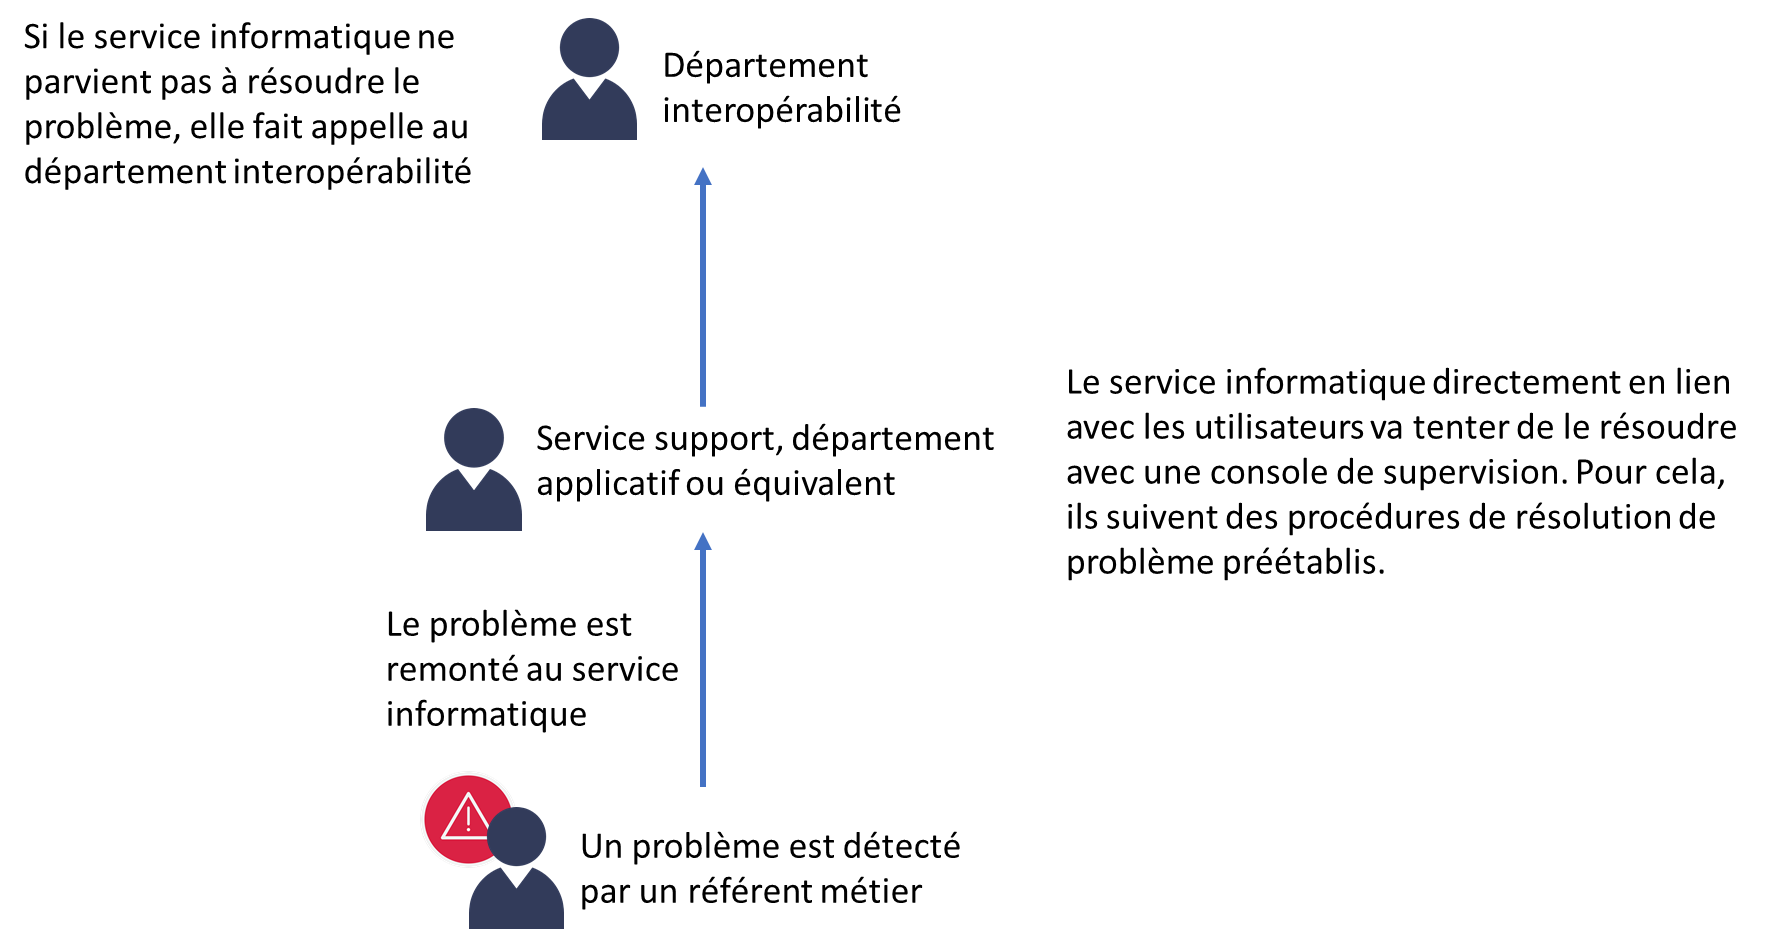
\includegraphics[width=15cm]{../img/user_1.png}
				\caption{\label{resolution_pbs} Processus de résolution d'un problème dans
				Cloverleaf.}
			\end{figure}
			
		\subsection{L'enquête permet de dresser la liste des besoins}
			\paragraph{}% Les attentes qui sont ressorties de l'enquête
			Les différentes personnes interrogées ont des avis similaires concernant le
			rôle des consoles de supervision. Elles attendent
			de ces outils qu’ils jouent le rôle d'un tableau de bord clair, simple et si
			possible au design épuré de façon à ce que les informations soient les plus
			lisibles possibles. Une console doit permettre une visualisation rapide des
			erreurs et leur compréhension. Leur correction n’est évoquée que comme une
			fonction secondaire et facultative de ces outils.\newline
			D’une manière générale, les utilisateurs sont satisfaits de l’ergonomie
			actuelle de TrackCIS et la cite comme un de ses points forts.
			Les principaux points négatifs sont~:
			\begin{itemize}
			  \item Le paramétrage des colonnes est difficile
			  \item La lenteur d’affichage des messages
			  \item Pour certains flux  (les flux externes), il faut parcourir l'ensemble
			  des messages pour retrouver ceux ayant eu un retour négatif
			\end{itemize}
			Les utilisateurs au profil informaticien ne sont pas spécialement sensibles
			à l’ergonomie des outils de supervision, mais sont plus soucieux de leurs
			fonctionnalités. Cependant le design et de la facilité de prise en main
			seraient des atouts plus importants pour des utilisateurs métiers.
			
			\paragraph{}% C'est quoi une bonne console
			En résumé, une bonne console est un outil donnant la vision la plus générale
			possible. La console de supervision a pour objectif premier de faire gagner
			du temps à son utilisateur et de permettre une résolution plus rapide des
			problèmes. De ce fait, la console de supervision a pour objectif d’améliorer
			la fiabilité globale de l’EAI, donc du SI.
			
			\paragraph{}% La lise des besoins, classification
			En plus des informations que nous avons décrites jusque-là, les entretiens
			nous ont permis d'identifier les besoins des utilisateurs. Ceux-ci ont été
			exprimés explicitement ou non, et concerne généralement des manques. Voici
			quelques exemples de besoins, la liste complète se trouvant en annexe C~:
			\begin{itemize}
			  \item Pouvoir trouver facilement la cause des erreurs
			  \item Voir l'évolution du nombre de messages envoyés par flux au cours du
			  temps
			  \item Voir la date et l'heure d'écriture du dernier message
			  \item Visualiser l'état des flux en temps réel
			  \item Pouvoir afficher la console sur un écran géant
			\end{itemize}
			Un total de 57 besoins a été ainsi identifiés. Ceux-ci ne sont pas
			spécifiquement liés à un outil, ils concernent la supervision
			en général. Certains de ces besoins sont déjà satisfaits dans
			TrackCIS, c'est par exemple le cas pour~: <<~Pouvoir rejouer les
			messages~>> ou encore <<~Avoir un outil utilisable en lecture seule~>>. Ce
			type de besoin nous ayant été remonté par des non utilisateurs de TrackCIS. Nous
			pouvons faire un premier classement des besoins en utilisant les catégories
			suivantes~:
			\begin{itemize}
			  \item Besoins concernant les performances
			  \item Besoins concernant le design, l'ergonomie et la facilité
			  d'utilisation
			  \item Besoins concernant la résolution des problèmes
			  \item Besoins concernant les données statistiques
			  \item Besoins concernant les rôles de la console
			  \item Les autres besoins
			\end{itemize}
			
			\paragraph{}% La lise des besoins, priorisation
			Le classement des besoins permet d'en faciliter la lecture et la
			compréhension, ce qui nous permettra d'imaginer plus aisément les
			fonctionnalités qui y répondront. Tous les éléments de cette
			liste ne sont pas égaux, certains besoins comptent d'avantage aux yeux des
			personnes interrogée que d'autre et certains ont été cités plus
			souvent.\newline
			De façon à noter l'importance de chaque besoin pour les utilisateurs, nous
			proposons de nous baser sur le barème présenté dans le tableau
			\ref{bareme_besoins} ainsi que sur le nombre de citations. Le choix des notes
			dans le barème ci-dessous a pour but
			de bien différencier les besoins les plus prioritaires de ceux qui le sont moins.
			\begin{table}[H]
				\centering
				\caption{\label{bareme_besoins} Barème choisi pour noter l'importance de
				chaque besoin perçu lors de l'entretien.}
				\begin{tabular}{| p{4cm} | p{8cm} | p{2cm} |}
					\hline
						\thead{Priorité}
						&\thead{Description}
						&\thead{Note}
						\\
					\hline
						Peu important
						&
						S'il est satisfait, ce besoin ne fait qu'améliorer le confort de l'utilisateur. S'il ne l'est pas, rien ne change.
						&
						2
						\\
					\hline
						Important
						&
						S'il est satisfait, améliore l'efficacité de l'utilisateur dans son
						métier.
						&
						3
						\\
					\hline
						Très important
						&
						S'il est satisfait, améliore considérablement l'efficacité de
						l'utilisateur dans son métier.
						&
						5
						\\
					\hline
						Critique
						&
						Besoin indispensable à satisfaire, faute de quoi cela nuira à l'utilisateur.
						&
						8
						\\
					\hline
				\end{tabular}
			\end{table}
			Nous calculons la note de chaque besoin avec la formule ci-dessous
			(formule \ref{besoin_formule}).
			Soit N le nombre de citation et I la note d'importance définie grâce au
			barème du tableau \ref{bareme_besoins}~:
			\begin{equation}
				\label{besoin_formule}
				Note\ du\ besoin=N\times I
			\end{equation}
			Le résultat de cette priorisation se trouve dans la colonne <<Note du besoin>>
			du tableau de l'annexe C.
	
	\section{La liste des besoins permet de dresser une liste de fonctionnalités}
		\paragraph{}% On ne se concentre que sur les besoins liés aux stats
		Nous avons dressé et analysé une liste de besoins émanant d'utilisateurs
		concernant la supervision en général. L'objectif est maintenant, à partir de
		cette liste, de dresser une liste de fonctionnalités pour TrackCIS.
		
		\subsection{De la liste des besoins à la liste des fonctionnalités}
			\paragraph{}% Mode de passage des besoins aux fonctionnalités
			Précisons tout d'abord que nous ne traiterons pas ici de tous les besoins de la
			liste, mais uniquement de ceux qui sont relatifs à un module d'affichage de
			statistiques. Xperis souhaite apporter toutes les améliorations nécessaires à
			TrackCIS. Cependant, l'amélioration prioritaire concerne le nouveau module
			statistique. C'est pourquoi les besoins relatifs aux statistiques seront
			les seuls à être traités ici, et donc à être déclinés en
			fonctionnalités.\newline
			Les éléments de cette liste qui ne seront pas traités dans ce mémoire
			pourront servir de base à Xperis pour des améliorations futures de l'outil.
		
			\paragraph{}% Une fonctionnalité est un service
			Une fonctionnalité est un service rendu par une application à un utilisateur.
			Par exemple, la version actuelle de TrackCIS permet à l'utilisateur de
			consulter la liste des messages qui sont passés dans un flux. Ceci est une
			fonctionnalité et elle répond à un besoin de l'utilisateur. En l'occurrence,
			le besoin en question pourrait être~: <<~je souhaite avoir accès à tous les
			messages qui transitent par mon flux~>>.
			Dans ce cas-ci, le passage du besoin à la fonctionnalité est simple. D’une
			façon générale un besoin n'est pas lié à un outil en particulier, c'est une
			volonté de l'utilisateur associée à un manque.
			Une fonctionnalité est quant à elle liée à un outil, il
			s'agit d'un service rendu par cet outil et qui répond à un besoin.
		
			\paragraph{}% La liste des fonctionalités
			On peut dresser une liste de 30 fonctionnalités (voir la liste
			complète en annexe D) à partir des 33 besoins que l'on a retenus. Nous
			regroupons en 8 grands ensembles \label{ensembles_fonctios}~:
			\begin{itemize}
			  \item Visualisation du niveau de disponibilité du flux.
			  \item Visualisation de la date et et de l'heure du dernier message passé.
			  \item Visualisation de l’historique des messages.
			  \item Visualisation des ressources serveur.
			  \item Administration des statistiques.
			  \item Exporter les données statistiques.
			  \item Facilitation de l’utilisation.
			\end{itemize}
			
		\subsection{Priorisation des fonctionnalités liées aux statistiques}
			\paragraph{}% But de la priorisation des fonctionnalités
			De la même manière que nous avons priorisé les besoins, nous cherchons ici à
			prioriser les fonctionnalités qui en découlent. L'objectif est
			d'anticiper leur développement~: les plus importantes
			devant être implémentées en premier. Il nous faut donc mettre en place un
			barème permettant d'ordonner les fonctionnalités par ordre d'importance. Nous
			allons nous aider pour cela du diagramme FODA (\textit{Feature oriented
			domain analysis}).
			
			\paragraph{}% Présentation FODA
			Le diagramme FODA est une représentation graphique des différentes
			fonctionnalités de l’application \citep{bontemps_semantics_2004}. Il est
			organisé en features.
			Une feature est une macro fonctionnalité. A l’intérieur de chaque feature
			peuvent se trouver d’autres fonctionnalités, plus précises, sous lesquelles
			peuvent s’en trouver d’autres, etc. Les feuilles de l’arbre ainsi formé
			(correspondant au niveau de fonctionnalité le plus détaillé) sont les parties
			fonctionnelles de l’application qui seront ensuite développées.\newline
			La figure \ref{foda_legende} présente le principe de base du diagramme FODA.
			La \textit{feature} 1 est obligatoire (point noir), elle correspond à la
			fonctionnalité d'un produit minimum viable (PMV), c'est-à-dire le produit le
			plus simple pouvant être commercialisé.
			La \textit{feature 2} est facultative (point blanc), elle correspond à une fonctionnalité qui pourra être
			développée dans des versions plus évoluées ou plus personnalisées de
			l’outil. Elle n’est pas indispensable au fonctionnement ni à la mise sur le
			marché, mais rend tout de même un service intéressant à l'utilisateur.
			\begin{figure}[H]% Légende du FODA
				\centering
				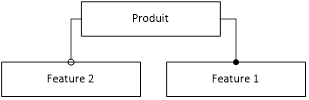
\includegraphics[width=7cm]{../img/foda_legende.png}
				\caption{\label{foda_legende} Principe du diagramme FODA}
			\end{figure}
			
			\paragraph{}% FODA de TrackCIS stats
			Nous mettons en pratique cette classification en concertation avec l'équipe
			d'Xperis. Cette séparation entre fonctionnalités optionnelles ou faisant
			parti du PMV reflète donc le choix de l'entreprise.
			Pour tenir également compte des priorités des utilisateurs interrogés durant
			l'enquête, il nous faut intégrer la note des besoins calculée précédemment.
			Une fonctionnalité est la réponse à un ou plusieurs besoins et un besoin peut
			être satisfait par plusieurs fonctionnalités (figure \ref{mapping_besoins}).
			Sachant cela, nous proposons la formule ci-dessous.
			Soit Bi la note d'un besoin donnée, \begin{math}\sum Bi\end{math} représente
			la somme des notes des besoins qui sont satisfaits par cette fonctionnalité.
			On a la formule \ref{fonctio_nopmv} pour une fonctionnalité notée comme
			facultative et la formule \ref{fonctio_pmv} pour une fonctionnalité notée
			comme obligatoire. Les notes obtenues pour chaque fonctionnalité sont
			présentées dans la colonne <<~Note de fonctionnalité~>> du tableau de
			l'annexe D.
			\begin{equation}
				\label{fonctio_nopmv}
				Note\ de\ la\ fonctionnalite=\sum Bi
			\end{equation}
			\begin{equation}
				\label{fonctio_pmv}
				Note\ de\ la\ fonctionnalite=2\times \sum Bi
			\end{equation}
			\begin{figure}[H]
				\centering
				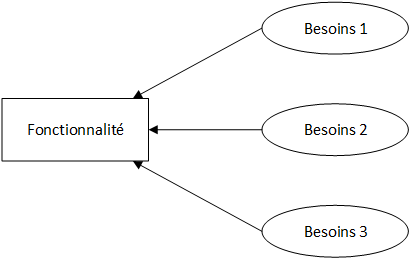
\includegraphics[width=7cm]{../img/part2/mapping_besoins.png}
				\caption{\label{mapping_besoins} Une fonctionnalité est la réponse à un ou
				plusieurs besoins}
			\end{figure}
			
		\subsection{Le nouveau module est découpé en huit grands groupes de
		fonctionnalités}
			\paragraph{}
			Les figures \ref{foda_1} et \ref{foda_2} représentent l'ensemble des
			fonctionnalités du module statistique de TrackCIS sous forme de diagramme FODA.
			Chaque \textit{feature} correspond à un des huit grands ensembles de
			fonctionnalités décrit à la page \pageref{ensembles_fonctios}.\newline
			La page dédiée aux statistiques serait divisée en widgets. Chacun est une
			petite boîte contenant un type d'information. Dans la version que nous
			proposons ici, ils sont au nombre de cinq et correspondent aux cinq premières
			\textit{features} décrites ci-dessous.
			\begin{figure}[H]% foda 1
				\centering
				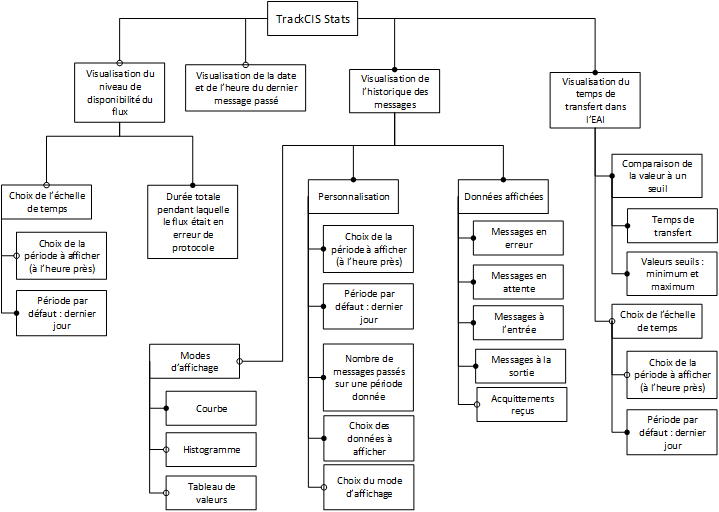
\includegraphics[width=16cm]{../img/part2/foda_1.png}
				\caption{\label{foda_1} Diagramme FODA pour le module statistique de
				TrackCIS (première partie)}
			\end{figure}
			\begin{figure}[H]% foda 2
				\centering
				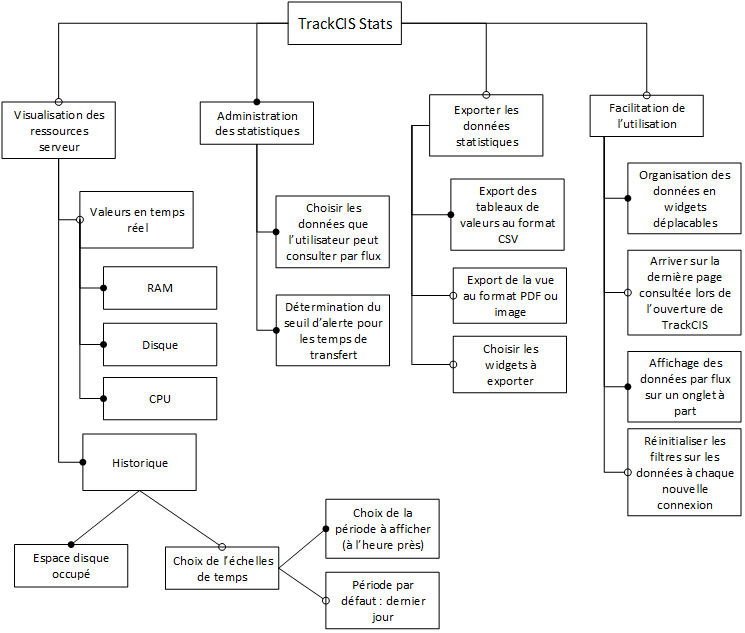
\includegraphics[width=16cm]{../img/part2/foda_2.png}
				\caption{\label{foda_2} Diagramme FODA pour le module statistique de
				TrackCIS (deuxième partie)}
			\end{figure}
			
			\paragraph{Visualisation du niveau de disponibilité du flux.}
			Cette \textit{feature} correspond au widget permettant d'afficher le taux de
			disponibilité du flux. Il s'agit du ratio entre le temps de bon
			fonctionnement du flux sur le temps où celui-ci ne fonctionnait pas pour
			causes d'erreurs. Cet indicateur permet de détecter rapidement les flux les
			plus problématiques. Cette valeur serait calculée sur une période de temps
			définie par l'utilisateur.
			
			\paragraph{Visualisation de la date et heure du dernier message passé.}
			Il s'agit d'une fonctionnalité toute simple mais que l'étude du besoin a fait
			ressortir comme importante. Il s'agit d'un petit widget indiquant avec
			précision la date et l'heure à laquelle un message est correctement passé
			pour la dernière fois sur ce flux. Ceci est un bon indicateur du bon
			fonctionnement d'un flux. Dans la plupart des flux hospitaliers, des messages
			passent en permanence. Le fait qu'il n'en passe pas pendant un certain temps
			est révélateur de problèmes.
			
			\paragraph{Visualisation de l’historique des messages.}
			Cette \textit{feature} correspond à un widget affichant l'historique du
			nombre de messages passés sur le flux. Celui-ci peut prendre la forme d'une courbe,
			d'un histogramme ou d'un simple tableau de valeurs. L'utilisateur choisi la
			période qu'il veut visualiser ainsi que les types de données. Ce widget
			permettrait de voir l'évolution au cours du temps des messages ayant
			correctement transité dans le flux, des messages tombés en erreurs ou en
			attente ou encore des acquittements reçuent des applications destinataires.
			
			\paragraph{Visualisation des ressources serveur.}
			Cette \textit{feature} correspond à deux widgets qui ont tous deux attraits à
			l'état du serveur sur lequel est installé Cloverleaf. Le premier d'entre eux permet
			d'avoir des informations sur l'état en temps réel du serveur~: occupation de
			la mémoire vive et du disque, utilisation du processeur. Le deuxième widget
			permet de voir l'évolution au cours du temps de l'occupation du disque du
			serveur. Cette donnée présentée sous la forme d'une courbe, peut permettre
			d'identifier une augmentation anormale de l'espace occupé, ce qui peut
			correspondre à une mauvaise gestion de la mémoire au niveau de l'EAI, ce qui
			peut poser problème à terme.\newline
			Les deux dernières features ne correspondent à aucun widget sur l'onglet
			statistiques.
			
			\paragraph{Administration des statistiques.}
			Cette partie est réservée aux administrateurs. Dans le
			PMV il est possible de définir quel utilisateur peut voir quel widget sur sa
			page statistique. Ce qui signifie que l'utilisateur ne peut pas paramétrer
			sa propre page, à part la position des widgets.
			
			\paragraph{Exporter les données statistiques.}
			L'utilisateur doit pouvoir exporter les données qu'il voit sur sa page
			statistique. L'export se fait donc pour un flux donné et dans divers formats.
			Dans le PMV, il est uniquement possible d'exporter les données sous forme de
			PDF ou d'image reprenant l'affichage du contenu des widgets à l'identique.
			Une version plus évoluée de la feature permettrait de choisir quelles sont
			les widgets que l'on veut exporter.
			
			\paragraph{Facilitation de l’utilisation.}
			Cette dernière feature concerne l'ergonomie que doit respecter le nouveau
			module. Celui-ci s'inscrit dans un outil existant, TrackCIS, dont
			la charte graphique est déjà bien établie. Cet outil se veut le plus facile à
			utiliser possible, le module statistique doit respecter cette philosophie.
	
	\section{Des fonctionnalités vers les cas d'utilisation}
		\paragraph{}
		Nous savons maintenant quelles sont les services que doit rendre notre nouveau
		module. Nous avons vu qu'ils ne sont pas tous destinés aux mêmes utilisateurs.
		Il en existe deux types pour TrackCIS~: les utilisateurs et les
		administrateurs. Le module statistique utilise aussi cette typologie. Les
		seules fonctionnalités décrites dans la partie précédente ne nous suffisent
		pas pour développer le module. A elles seules, elles décrivent d'une certaine
		manière le futur module, mais ça n'est pas suffisant. Il nous faut une
		description plus précise et surtout dynamique de la solution, ce que nous
		obtiendrons grâce aux maquettes.
		
		\subsection{État de l'art sur les consoles de supervision et la visualisation de données}
			\paragraph{}
			L'objectif de l'état de l'art est de s'inspirer de ce qui existe par
			ailleurs.
			Ici, nous analyserons des outils remplissant des
			fonctions similaires à celles que l’on attendrait de TrackCIS. Pour chaque
			outil étudié, nous nous attarderons sur~:
			\begin{itemize}
			  \item Les données qui sont affichées et leurs rôles respectifs (ce qu'elles
			  apportent à l'utilisateur),
			  \item La manière dont ces données sont représentées (courbe, histogramme,
			  jauge...), pourquoi elles sont représentées de la sorte et si cela semble
			  efficace et ergonomique du point de vue de l’utilisateur.
			\end{itemize}
			Nous analyserons ici 2 outils~: TradeXpress et M12.
			
			\paragraph{TradeXpress~:}
			TradeXpress est une plateforme d’intégration B2B (Business to business)
			\citep{gmi_connectivity_gateway_2014}.
			Elle permet de connecter les applications d’une entreprise à celles de ses
			partenaires (clients, fournisseurs…). TradeXpress n’est pas spécialisée dans
			un domaine en particulier et permet de gérer l’intégralité des flux entre
			applications, allant bien au-delà de la simple supervision. Cependant, certaines
			de ces fonctionnalités sont axées supervision, ce sont celles qui nous
			intéressent ici. La figure \ref{trade_xpress} présente la page de monitoring des
			flux.\newline
			La vue est divisée en deux parties aux rôles
			différents~: l'une (à gauche) est consacrée à l’état du système, l'autre (à
			droite) à la supervision. La première partie montre une vision de l’état
			actuel (en temps réel) du serveur avec des informations comme l'espace
			disque disponible ou l'occupation de la mémoire vive.
			La partie supervision présente deux types d'informations~:
			\begin{itemize}
			  \item Une vue au jour à l’aide de jauges montrant le nombre de messages ou
			  documents transitant par la plateforme. On peut voir juste en-dessous de
			  l’encadré gris un bouton permettant de choisir la date.
			  \item Un historique à la semaine du volume de messages passé pour chaque
			  domaine métier (commandes, factures\ldots). L’utilisateur peut choisir les
			  données ainsi que la semaine à afficher.
			\end{itemize}
			Le design de l’outil est simple et relativement classique. Les informations
			utiles à l’utilisateur occupent un maximum de place sur la page. Il y a peu
			de superflu~: pas de cadre autour des parties et seulement cinq couleurs différentes.\newline
			Pour la partie supervision, l’utilisateur ne peut pas sélectionner la
			période de temps, il doit se contenter de visualiser les données d’un jour
			ou d’une semaine. Ceci restreint les possibilités de
			visualisation, mais simplifie l’utilisation de la console.\newline
			Pour que les jauges soient pertinentes il faut qu’elles soient calibrées avec
			une valeur minimum et maximum. La documentation disponible en ligne ne précise
			pas s’il est possible de calibrer ces jauges, ni à qui revient ce rôle.
			\begin{figure}[H]
				\centering
				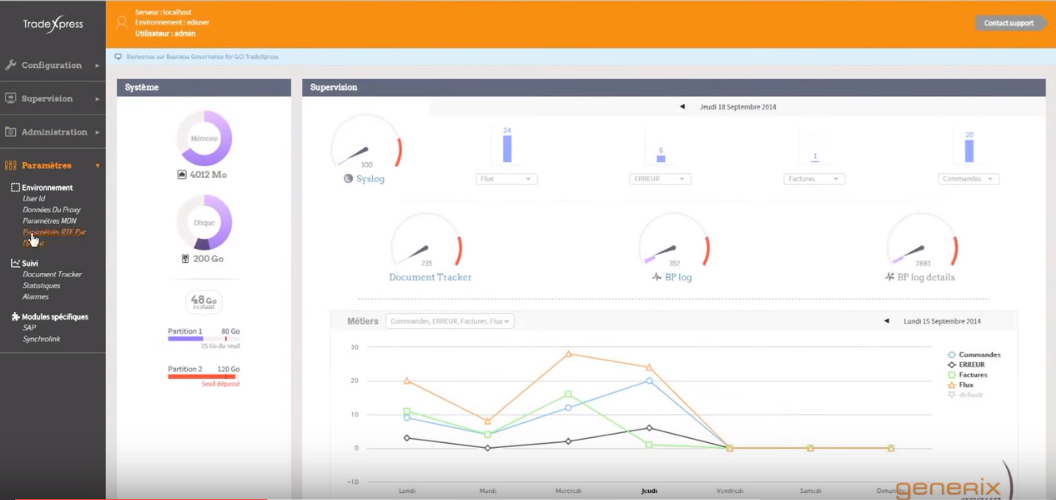
\includegraphics[width=16cm]{../img/part2/trade_xpress.png}
				\caption{\label{trade_xpress} Tableau de bord de l'outil Trade Xpress.}
			\end{figure}
			
			\paragraph{M12~:}
			M12 est également une console permettant de surveiller des flux de données
			\citep{processmview_m12}, principalement des flux basés sur des services web.
			Elle permet notamment de générer des alertes (par exemple des alertes envoyées par mail) en cas de
			problème et de rejouer les messages.\newline
			L'interface est présentée par la figure \ref{m12}. Peu d'informations sout
			librement accessibles sur cet outil, c'est pourquoi nous ne nous attarderons
			que sur les trois graphiques situés dans la partie gauche de la page.
			Chacun apporte deux informations, l'une se situe à l'intérieur du cercle
			gris sous la forme d'un nombre, l'autre en dehors du cercle sous la forme
			d'un pourcentage. Le cercle en soi n'apporte pas d'informations à
			l'utilisateur.\newline
			Les informations sont réparties sur la page sous la
			forme d'encadré contenant chacun un type de données.
			\begin{figure}[H]
				\centering
				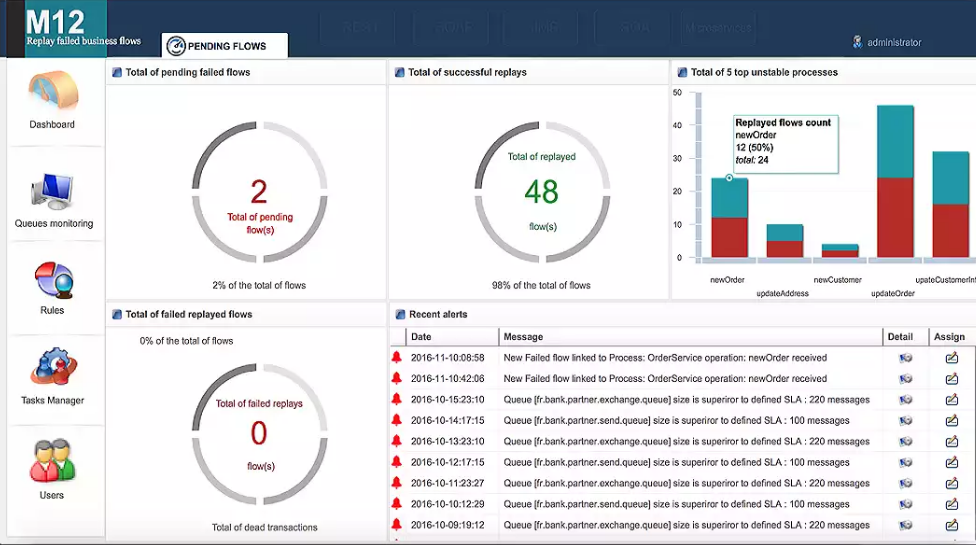
\includegraphics[width=16cm]{../img/part2/m12.png}
				\caption{\label{m12} Tableau de bord de l'outil M12.}
			\end{figure}
			
			\paragraph{}
			A la suite de cet état de l'art, les idées suivantes peuvent être retenues
			pour TrackCIS~:
			\begin{itemize}
			  \item l'utilisation de compteurs ou de jauges est pertinente pour
			  visualiser des données en temps réel, comme par exemple l'utilisation de
			  la mémoire vive d'un serveur. Cela nécessite d'avoir une valeur minimum et
			  une valeur de seuil pour que l'utilisateur puisse interpréter rapidement la
			  donnée qui lui est présentée.
			  \item Chaque élément présent dans une visualisation doit contribuer à
			  apporter une information à l'utilisateur.
			  \item Moins l'utilisateur doit faire de clics pour afficher les
			  informations qu'il veut, mieux c'est. C'est par exemple le cas d'un tableau
			  de bord présentant en une seule page de multiples données <<~prêtes à
			  l'usage~>>.
			  \item Donner trop de libertés à l'utilisateur peut en complexifier
			  l'expérience. Il peut être judicieux de restreindre, par exemple, le choix
			  des périodes de temps ou le choix des données à afficher sur un graphique.
			\end{itemize}
			
		\subsection{Création de scénarios d'utilisation illustrés à l'aide de
		maquettes}
			\paragraph{}
			A partir des fonctionnalités et des idées collectées dans l'état de l'art,
			nous pouvons commencer à décrire plus précisément le futur outil grâce à des
			maquettes. Pour les présenter, nous utiliserons un scénario d'utilisation.
			Nous nous placerons dans le cas d'un administrateur souhaitant superviser un
			flux et autoriser un utilisateur à voir des statistiques pour ce flux.
			
			\paragraph{Vue utilisateur~:}
			L'administrateur se connecte à son compte TrackCIS et se rend sur l'onglet
			statistique (point (1) sur la figure \ref{maquette_user}). C'est sur cette
			page qu'il peut consulter un certain nombre de données sur chaque flux. Il
			sélectionne (2) celui qui l'intéresse, en l'occurrence le flux nommé
			<<~HPRIM~>>.
			Ce faisant, les données qui s'affichent sur la page sont relatives à ce flux.
			L'administrateur consulte tout d'abord la date et l'heure de passage du
			dernier message (3) pour s'assurer que le flux n'est pas bloqué. Il consulte ensuite
			l'historique du nombre de messages en entrée et en sortie dans le widget
			juste en-dessous (4). Ce graphique lui permet éventuellement de détecter des
			tendances anormales à moyen et à long terme. Enfin, il consulte le temps de
			transfert moyen d'un message à l'aide de la jauge (5). Le fait que cette
			valeur moyenne soit trop élevée peut être révélateur de problèmes. A ce
			niveau, l'administrateur a terminé son travail de supervision, il clique sur
			l'onglet <<~Droits~>> puis sur <<~Statistiques~>> pour gérer les droits des
			utilisateurs.
			\begin{figure}[H]
				\centering
				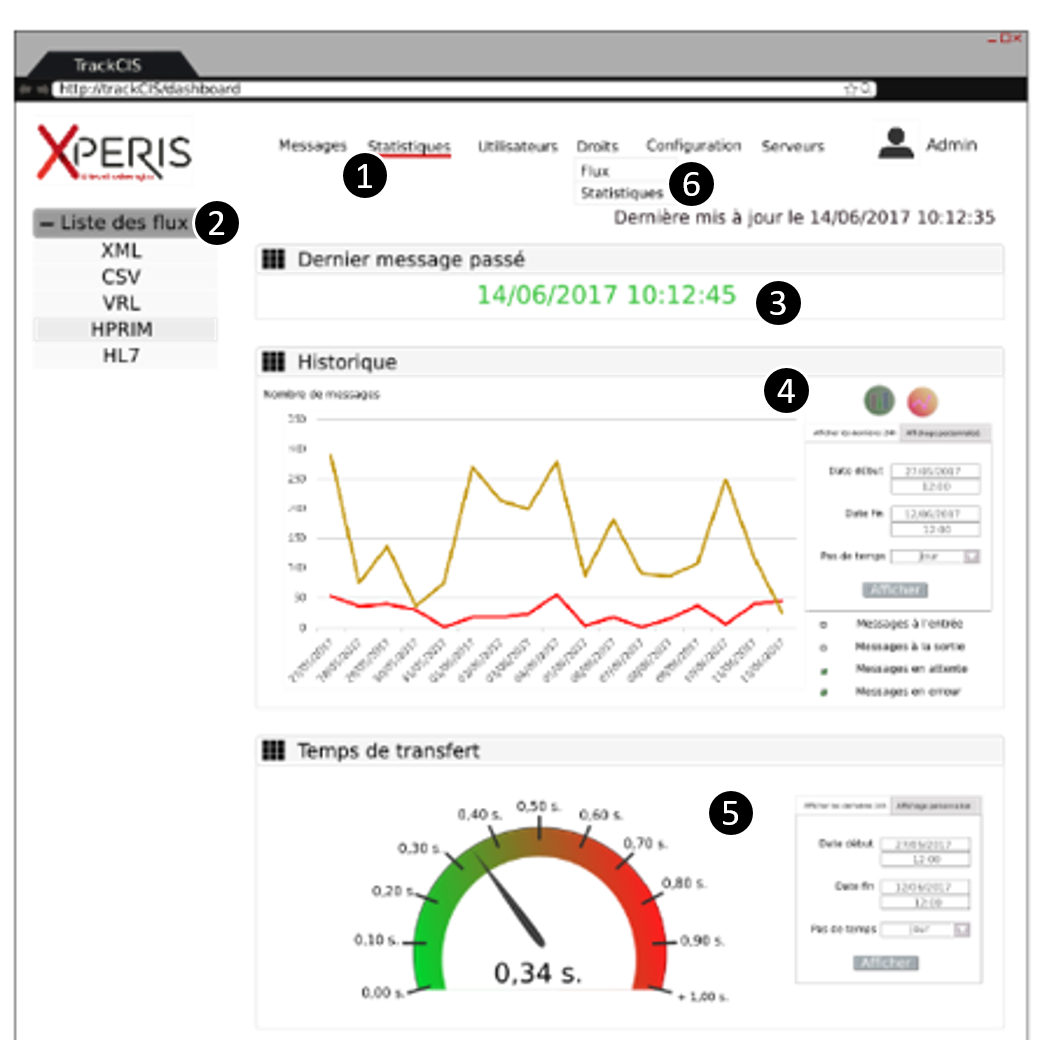
\includegraphics[width=16cm]{../img/part2/maquette_user_1.png}
				\caption{\label{maquette_user} Maquette de l'onglet statistique de
				TrackCIS.}
			\end{figure}
			
			\paragraph{Vue administrateur~:}
			L'administrateur arrive sur la page de gestion des droits pour les
			statistiques. Il commence par choisir l'utilisateur de qui il souhaite
			modifier les droits (point (7) de la figure \ref{maquette_admin}). A l'aide
			de boutons radio, il peut autoriser l'affichage d'un widget donné pour un
			flux donné pour l'utilisateur sélectionné (8). C'est donc l'administrateur
			et lui seul qui peut personnaliser l'affichage des statistiques de tous les
			utilisateurs de TrackCIS.
			\begin{figure}[H]
				\centering
				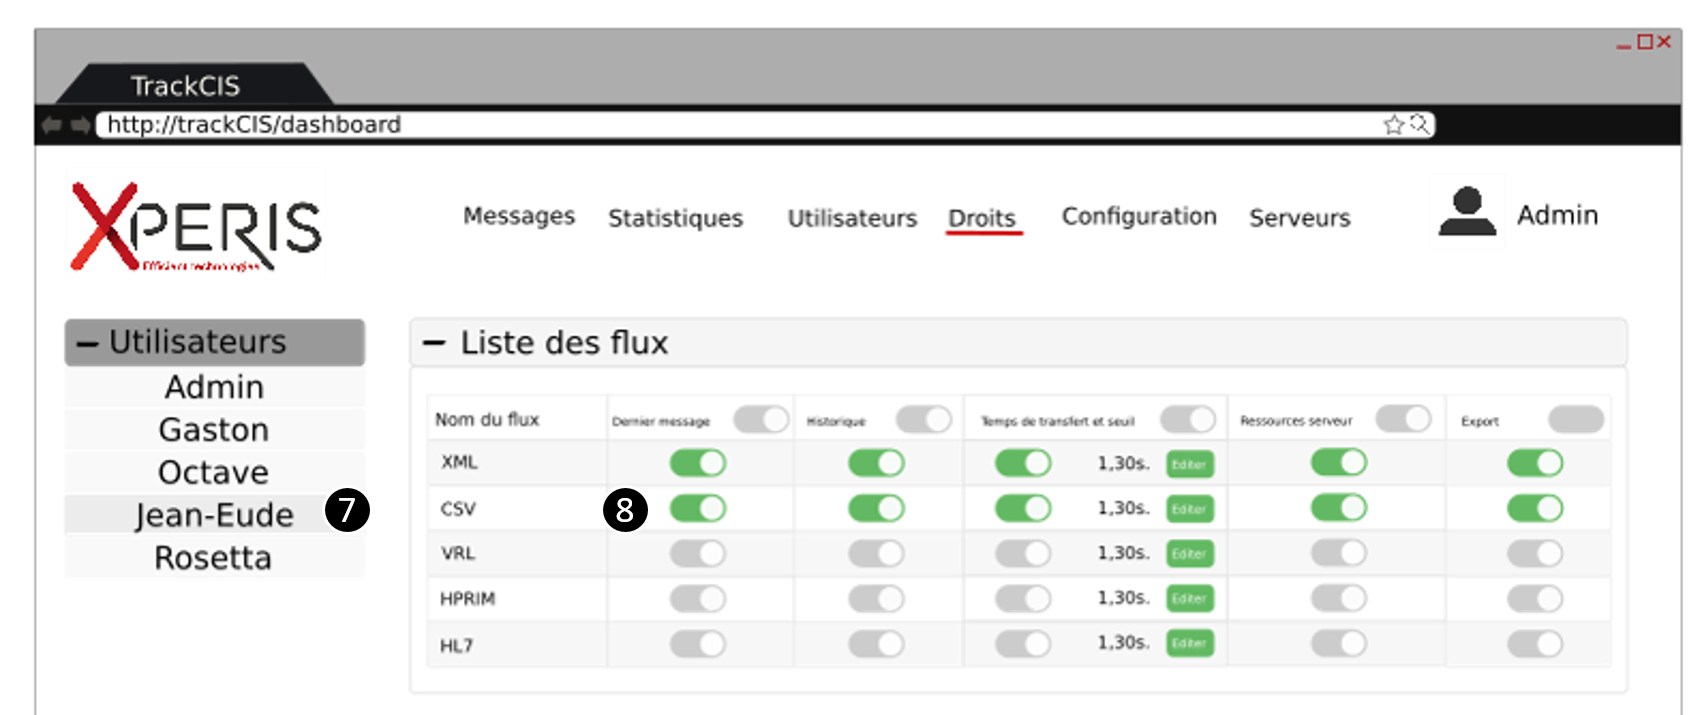
\includegraphics[width=16cm]{../img/part2/maquette_admin_1.png}
				\caption{\label{maquette_admin} Maquette de l'onglet permettant
				l'administration des statistiques de TrackCIS.}
			\end{figure}
			